% Written By Enoch Yu
% Downloaded from archive.enochyu.com

\documentclass{article}

\usepackage{amsmath,amsthm,amssymb}

\usepackage{tikz}
\usetikzlibrary{calc}

\usepackage{parskip}
\usepackage[margin=1in]{geometry}
\usepackage[font=small,labelfont=bf]{caption}
\usepackage{float}
\usepackage{enumitem}

\usepackage{fancyhdr}
\pagestyle{fancy}
\fancyhead[R]{Enoch Yu}
\fancyhead[L]{Trigonometric Identities}


\newtheorem{theorem}{Theorem}[section]
\newtheorem{lemma}[theorem]{Lemma}
\newtheorem{sublemma}{Lemma}[section]
\newtheorem{proposition}{Proposition}
\newtheorem{corollary}{Corollary}[theorem]
\newenvironment{solution}{\begin{trivlist}\item[]{\bf Solution}}
    {\qed \end{trivlist}}


\title{Trigonometric Identities}
\author{Enoch Yu}
\date{30 April 2025}


\begin{document}

\maketitle

\tableofcontents

\newpage
% Section 1
\section{List of Relationships and Formulas}
\begin{enumerate}
\item
$\sin(\alpha + \beta)
= \sin\alpha \cos\beta + \cos\alpha\sin\beta$
%
\item
$\cos(\alpha + \beta)
= \cos\alpha \cos\beta - \sin\alpha \sin\beta$
%
\item
$\tan(\alpha + \beta)
= \frac{\tan\alpha + \tan\beta}{1 - \tan\alpha \tan\beta}$
%
\item
$\sin(\alpha - \beta)
= \sin\alpha \cos\beta - \cos\alpha \sin\beta$
%
\item
$\cos(\alpha - \beta)
= \cos\alpha \cos\beta + \sin\alpha \sin\beta$
%
\item
$\tan(\alpha - \beta)
= \frac{\tan\alpha - \tan\beta}{1 + \tan\alpha \tan\beta}$
%
\item
$\sin2\alpha
= 2\sin\alpha \cos\alpha
=\frac{2\tan\alpha}{1 + \tan^2\alpha}$
%
\item
$\cos2\alpha
= \cos^2\alpha - \sin^2\alpha
= 2\cos^2\alpha - 1
= 1 - 2\sin^2\alpha
= \frac{1 - \tan^2\alpha}{1 + \tan^2\alpha}$
%
\item
$\tan2\alpha
= \frac{2\tan\alpha}{1 - \tan^2\alpha}$
%
\item
$\sin3\alpha
= 3\sin\alpha - 4\sin^3\alpha$
%
\item
$\cos3\alpha
= 4\cos^3\alpha - 3\cos\alpha$
%
\item
$\sin\frac{\alpha}{2}
= \pm\sqrt{\frac{1 - \cos\alpha}{2}}$
%
\item
$\cos\frac{\alpha}{2}
= \pm\sqrt{\frac{1 + \cos\alpha}{2}}$
%
\item
$\tan\frac{\alpha}{2}
= \pm\sqrt{\frac{1 - \cos\alpha}{1 + \cos\alpha}}
= \frac{\sin\alpha}{1 + \cos\alpha}
= \frac{1 - \cos\alpha}{\sin\alpha}$
%
\item
$\sin\theta
= \frac{2\tan\frac{\theta}{2}}{1 + \tan^2\frac{\theta}{2}}$
%
\item
$\cos\theta
= \frac{1 - \tan^2\frac{\theta}{2}}
    {1 + \tan^2\frac{\theta}{2}}$
%
\item
$\tan\theta
= \frac{2\tan\frac{\theta}{2}}
    {1 - \tan^2\frac{\theta}{2}}$
%
\item
$\sin\alpha + \sin\beta
= 2\sin\frac{\alpha + \beta}{2}
    \cos\frac{\alpha - \beta}{2}$
%
\item
$\sin\alpha - \sin\beta
= 2\cos\frac{\alpha + \beta}{2}
    \sin\frac{\alpha - \beta}{2}$
%
\item
$\cos\alpha + \cos\beta
= 2\cos\frac{\alpha + \beta}{2}
    \cos\frac{\alpha - \beta}{2}$
%
\item
$\cos\alpha - \cos\beta
= -2\sin\frac{\alpha + \beta}{2}
    \sin\frac{\alpha - \beta}{2}$
%
\item
$\sin\alpha \cos\beta
= \frac{1}{2} [
    \sin(\alpha + \beta) + \sin(\alpha - \beta)
]$
%
\item
$\cos\alpha \sin\beta
= \frac{1}{2} [
    \sin(\alpha + \beta) - \sin(\alpha - \beta)
]$
%
\item
$\cos\alpha \cos\beta
= \frac{1}{2} [
    \cos(\alpha + \beta) + \cos(\alpha - \beta)
]$
%
\item
$\sin\alpha \sin\beta
= -\frac{1}{2} [
    \cos(\alpha + \beta) - \cos(\alpha - \beta)
]$
%
\item
$\sin^2\alpha = \frac{1}{2} (1 - \cos2\alpha)$
%
\item
$\cos^2\alpha = \frac{1}{2} (1 + \cos2\alpha)$
\end{enumerate}


% Section 2
\section{Angle Sum Relationships}
\subsection{List of Relationships}
\begin{align*}
    \sin(\alpha + \beta)
    &= \sin\alpha \cos\beta + \cos\alpha \sin\beta \\
    \cos(\alpha + \beta)
    &= \cos\alpha \cos\beta - \sin\alpha \sin\beta \\
    \tan(\alpha + \beta)
    &= \frac{\tan\alpha + \tan\beta}{1 - \tan\alpha \tan\beta}
\end{align*}

\subsection{Relationship for $\sin(\alpha + \beta)$}
\[
\sin(\alpha + \beta)
= \sin\alpha \cos\beta + \cos\alpha \sin\beta
\]
\begin{proof}
Consider the diagram below.

\begin{center}
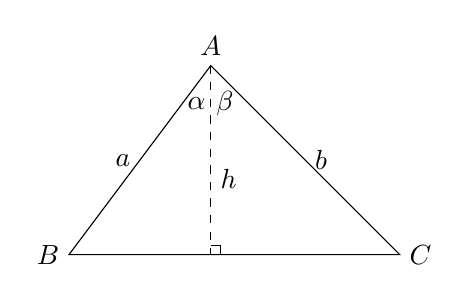
\begin{tikzpicture}[scale=0.6]
    \coordinate (A) at (0,0);
    \coordinate (B) at (7,0);
    \coordinate (C) at (3,4);
    \coordinate (D) at (3,0);

    \draw (A) -- (C) -- (B) -- cycle;
    \draw[dashed] (C) -- (D);
    \draw (3.2,0) -- (3.2,0.2) -- (3,0.2);

    \node[left] at ($(A)!0.5!(C)$) {$a$};
    \node[right] at ($(B)!0.5!(C)$) {$b$};
    \node[right] at ($(C)!0.6!(D)$) {$h$};
    \node at ($(C) + (-0.3,-0.8)$) {$\alpha$};
    \node at ($(C) + (0.3,-0.8)$) {$\beta$};

    \node[left] at (A) {$B$};
    \node[right] at (B) {$C$};
    \node[above] at (C) {$A$};
\end{tikzpicture}
\end{center}

It is evident that $h = a\cos\alpha = b\cos\beta$
because $\cos\alpha = \frac{a}{y}$ and
$\cos\beta = \frac{b}{y}$.
Using the area formula of triangle, the following
equation is true.
\[
\frac{1}{2} ab \sin(\alpha + \beta)
= \frac{1}{2} ah \sin\alpha + \frac{1}{2} bh \sin\beta
\]
$h$ could be replaced with $b\cos\beta$ and
$a\cos\alpha$ respectively.
\[
\frac{1}{2} ab \sin(\alpha + \beta)
= \frac{1}{2} ab \cos\beta \sin\alpha +
    \frac{1}{2} ba \cos\alpha \sin\beta
\]
By multiplying both sides by two and dividing by
$ab$ (because $ab \neq 0$), the following relationship
may be obtained. Moreover, despite the fact that the
current proof is not feasible for the case where
$ab = 0$, the relationship appears to be true for
$ab = 0$ also. 
\[
\therefore \sin(\alpha + \beta)
= \sin\alpha \cos\beta + \cos\alpha \sin\beta
\]
\end{proof}

\subsection{Relationship for $\cos(\alpha + \beta)$}
\[
\cos(\alpha + \beta)
= \cos\alpha \cos\beta - \sin\alpha \sin\beta
\]
\begin{proof}
Let $\alpha = \frac{\pi}{2} + \gamma$. $\alpha$ could
be substituted for $\sin(\alpha + \beta) =
\sin\alpha \cos\beta + \cos\alpha \sin\beta$. The
following equation is obtained.
\[
\sin(\frac{\pi}{2} + \gamma + \beta)
= \sin(\frac{\pi}{2} + \gamma) \cos\beta
    + \cos(\frac{\pi}{2} + \gamma) \sin\beta
\]
Using the properties of trigonometric functions,
$\sin(\frac{\pi}{2} + \gamma) = \cos\gamma$ and
$\cos(\frac{\pi}{2} + \gamma) = -\sin\gamma$ are true.
\[
\therefore \sin(\frac{\pi}{2} + \gamma) \cos\beta +
    \cos(\frac{\pi}{2} + \gamma) \sin\beta
= \cos\gamma \cos\beta - \sin\gamma \sin\beta
\]
In another words, $\sin(\frac{\pi}{2} + \gamma + \beta)
= \cos(-\gamma - \beta) = \cos(\gamma + \beta)
= \cos\gamma \cos\beta - \sin\gamma \sin\beta$ is true.
The equation could be rewritten by changing the variables
to adhere to convention in using variables:
\[
\therefore \cos(\alpha + \beta)
= \cos\alpha \cos\beta - \sin\alpha \sin\beta.
\]
\end{proof}

%%%%%%%%%%%%%%%%%%%%%%%%%%%%%%%%%%%%%%%%%%%%%%%%%
%%%%%%%%%%%%%%%%%%%%%%%%%%%%%%%%%%%%%%%%%%%%%%%%%

\subsection{Relationship for $\tan(\alpha+\beta)$}
\[
\tan(\alpha+\beta)=\frac{\tan\alpha+\tan\beta}{1-\tan\alpha\tan\beta}
\]
\begin{proof}
    $\tan(\alpha+\beta)$ could be rewritten as $\frac{\sin(\alpha+\beta)}{\cos(\alpha+\beta)}$ by definition. Moreover, because $\sin(\alpha+\beta)=\sin\alpha\cos\beta+\cos\alpha\sin\beta$ and $\cos(\alpha+\beta)=\cos\alpha\cos\beta-\sin\alpha\sin\beta$, it is evident that
    \[
    \frac{\sin(\alpha+\beta)}{\cos(\alpha+\beta)}=\frac{\sin\alpha\cos\beta+\cos\alpha\sin\beta}{\cos\alpha\cos\beta-\sin\alpha\sin\beta}
    \] is true. $\cos\alpha\cos\beta$ could be factored from both the numerator and the denominator.
    \[
    \frac{\sin\alpha\cos\beta+\cos\alpha\sin\beta}{\cos\alpha\cos\beta-\sin\alpha\sin\beta}=\frac{(\cos\alpha\cos\beta)(\frac{\sin\alpha}{\cos\alpha}+\frac{\sin\beta}{\cos\beta})}{(\cos\alpha\cos\beta)(1-\frac{\sin\alpha\sin\beta}{\cos\alpha\cos\beta})}
    \]
    The terms may be organized with different forms.
    \[
    \frac{(\cos\alpha\cos\beta)(\frac{\sin\alpha}{\cos\alpha}+\frac{\sin\beta}{\cos\beta})}{(\cos\alpha\cos\beta)(1-\frac{\sin\alpha\sin\beta}{\cos\alpha\cos\beta})}=\frac{\tan\alpha+\tan\beta}{1-\tan\alpha\tan\beta}
    \]
    Therefore, the following expression is true.
    \[
    \tan(\alpha+\beta)=\frac{\tan\alpha+\tan\beta}{1-\tan\alpha\tan\beta}
    \]
\end{proof}

% Section 3
\section{Angle Difference Relationships}
\subsection{List of Relationships}
\begin{align*}
    \sin(\alpha-\beta)&=\sin\alpha\cos\beta-\cos\alpha\sin\beta \\
    \cos(\alpha-\beta)&=\cos\alpha\cos\beta+\sin\alpha\sin\beta \\
    \tan(\alpha-\beta)&=\frac{\tan\alpha-\tan\beta}{1+\tan\alpha\tan\beta}
\end{align*}

\subsection{Relationship for $\sin(\alpha-\beta)$}
\[
\sin(\alpha-\beta)=\sin\alpha\cos\beta-\cos\alpha\sin\beta
\]
\begin{proof}
The equation $\sin(\alpha + \beta) =
\sin\alpha \cos\beta + \cos\alpha\sin\beta$
is proven to be true.

Substitute $-b$ instead of $b$ to obtain
$\sin(\alpha - \beta) = \sin\alpha \cos(-\beta) +
\cos\alpha \sin(-\beta) = \sin\alpha \cos\beta -
\cos\alpha\sin\beta$.
\[
\therefore \sin(\alpha - \beta)
= \sin\alpha \cos\beta - \cos\alpha\sin\beta
\]
\end{proof}

\subsection{Relationship for $\cos(\alpha-\beta)$}
\[
\cos(\alpha-\beta)=\cos\alpha\cos\beta+\sin\alpha\sin\beta
\]
\begin{proof}
$\cos(\alpha + \beta) = \cos\alpha \cos\beta -
\sin\alpha\sin\beta$ is proven to be true.

Substitute $-b$ instead of $b$ to obtain
$\cos(\alpha - \beta) = \cos\alpha \cos(-\beta) -
\sin\alpha \sin(-\beta) = \cos\alpha \cos\beta +
\sin\alpha\sin\beta$.
\[
\therefore \cos(\alpha - \beta)
= \cos\alpha \cos\beta + \sin\alpha\sin\beta
\]
\end{proof}

\subsection{Relationship for $\tan(\alpha-\beta)$}
\[
\tan(\alpha-\beta)=\frac{\tan\alpha-\tan\beta}{1+\tan\alpha\tan\beta}
\]
\begin{proof}
$\tan(\alpha + \beta) =
\frac{\tan\alpha + \tan\beta}{1 - \tan\alpha \tan\beta}$
is proven to be true.

Substitute $-b$ instead of $b$ to obtain
$\tan(\alpha - \beta)
= \frac{\tan\alpha + \tan(-\beta)}{1-\tan\alpha \tan(-\beta)}
= \frac{\tan\alpha - \tan\beta}{1 + \tan\alpha \tan\beta}$.
\[
\therefore
\tan(\alpha - \beta)
= \frac{\tan\alpha - \tan\beta}{1 + \tan\alpha \tan\beta}
\]
\end{proof}


% Section 4
\section{Double Angle Relationships}
\subsection{List of Relationships}
\begin{align*}
    \sin2\alpha&=2\sin\alpha\cos\alpha \\
    &=\frac{2\tan\alpha}{1+\tan^2\alpha} \\\\
    \cos2\alpha&=\cos^2\alpha-\sin^2\alpha \\
    &=2\cos^2\alpha-1 \\
    &=1-2\sin^2\alpha \\
    &=\frac{1-\tan^2\alpha}{1+\tan^2\alpha} \\\\
    \tan2\alpha&=\frac{2\tan\alpha}{1-\tan^2\alpha}
\end{align*}

\subsection{Relationship for $\sin2\alpha$}
    \[
    \sin2\alpha=2\sin\alpha\cos\alpha
    \]
\begin{proof}
    Substitute $\alpha$ instead of $\beta$ in the proven equation:
    $\sin(\alpha+\beta)=\sin\alpha\cos\beta+\cos\alpha\sin\beta$.
    \[
    \sin(\alpha+\alpha)=\sin\alpha\cos\alpha+\cos\alpha\sin\alpha
    \]
    Therefore, the following equation is true.
    \[
    \sin2\alpha=2\sin\alpha\cos\alpha
    \]
\end{proof}
    \[
    \sin2\alpha=\frac{2\tan\alpha}{1+\tan^2\alpha}
    \]
\begin{proof}
    $\tan2\alpha$ could be rewritten to use the formulas that would later be proven.
    \[
    \tan2\alpha=\frac{\sin(2\alpha)}{\cos(2\alpha)}=\frac{2\tan\alpha}{1-\tan^2\alpha}
    \]
    $\cos2\alpha$ could be multiplied to both sides.
    \[
    \sin2\alpha=\frac{2\tan\alpha}{1-\tan^2\alpha}\cdot\cos2\alpha=\frac{2\tan\alpha}{1-\tan^2\alpha}\cdot\frac{1-\tan^2\alpha}{1+\tan^2\alpha}
    \]
    The following equation is resulted.
    \[
    \sin2\alpha=\frac{2\tan\alpha}{1+\tan^2\alpha}
    \]
\end{proof}

\subsection{Relationship for $\cos2\alpha$}
\begin{align*}
    \cos2\alpha&=\cos^2\alpha-\sin^2\alpha \\
    &=2\cos^2\alpha-1 \\
    &=1-2\sin^2\alpha
\end{align*}
\begin{proof}
    Substitute $\alpha$ instead of $\beta$ in the proven equation:
    $\cos(\alpha+\beta)=\cos\alpha\cos\beta-\sin\alpha\sin\beta$.
    \[
    \cos(\alpha+\alpha)=\cos\alpha\cos\alpha-\sin\alpha\sin\alpha
    \]
    Therefore, the following equation is true.
    \[
    \cos2\alpha=\cos^2\alpha-\sin^2\alpha
    \]
    Using Pythagorean Trigonometric Identity, the equation could be further modified.
    \[
    \cos2\alpha=\cos^2\alpha-\sin^2\alpha=2\cos^2\alpha-1=1-2\sin^2\alpha
    \]
\end{proof}
    \[
    \cos2\alpha=\frac{1-\tan^2\alpha}{1+\tan^2\alpha}
    \]
\begin{proof}
    It is evident that $\cos(2\alpha)=\cos^2\alpha-\sin^2\alpha$ is true. The equation could be modified to factor $\cos^2\alpha$ from both numerator and denominator.
    \begin{align*}
    \cos2\alpha&=\cos^2\alpha-\sin^2\alpha \\
    &=\frac{\cos^2\alpha-\sin^2\alpha}{1} \\
    &=\frac{\cos^2\alpha-\sin^2\alpha}{\cos^2\alpha+\sin^2\alpha} \\
    &=\frac{(\cos^2\alpha)(1-\frac{\sin^2\alpha}{\cos^2\alpha})}{(\cos^2\alpha)(1+\frac{\sin^2\alpha}{\cos^2\alpha})} \\
    &=\frac{1-\tan^2\alpha}{1+\tan^2\alpha}
    \end{align*}
    \[
    \therefore \cos2\alpha=\frac{1-\tan^2\alpha}{1+\tan^2\alpha}
    \]
\end{proof}

\subsection{Relationship for $\tan2\alpha$}
\[
\tan2\alpha=\frac{2\tan\alpha}{1-\tan^2\alpha}
\]
\begin{proof}
    Substitute $\alpha$ instead of $\beta$ in the proven equation:
    $\tan(\alpha+\beta)=\frac{\tan\alpha+\tan\beta}{1-\tan\alpha\tan\beta}$.
    \[
    \tan(\alpha+\alpha)=\frac{\tan\alpha+\tan\alpha}{1-\tan\alpha\tan\alpha}
    \]
    Therefore, the following equation is true.
    \[
    \tan2\alpha=\frac{2\tan\alpha}{1-\tan^2\alpha}
    \]
\end{proof}


% Section 5
\section{Triple Angle Formulas}
\subsection{List of Formulas}
\begin{align*}
    \sin3\alpha&=3\sin\alpha-4\sin^3\alpha \\
    \cos3\alpha&=4\cos^3\alpha-3\cos\alpha
\end{align*}
\noindent
Addition and double angle formulas may be utilized to derive triple angle formulas.

\subsection{Formula for $\sin3\alpha$}
    \[
    \sin3\alpha=3\sin\alpha-4\sin^3\alpha
    \]
\begin{proof}
    $\sin3\alpha$ may be rewritten as $\sin(2\alpha+\alpha)$. $\sin(2\alpha+\alpha)=\sin(2\alpha)\cos\alpha+\cos(2\alpha)\sin\alpha$ could be obtained by using addition relationship. The expression could be further modified through using double angle relationship.
    \[
    \sin(2\alpha)\cos\alpha+\cos(2\alpha)\sin\alpha=2\sin\alpha\cos^2\alpha+(\cos^2\alpha-\sin^2\alpha)\sin\alpha
    \]
    $2\sin\alpha\cos^2\alpha+(\cos^2\alpha-\sin^2\alpha)\sin\alpha=3\sin\alpha\cos^2\alpha-\sin^3\alpha$ could be obtained through rearrangement of terms. Pythagorean trigonometric identities could be utilized to further simplify the equation by using only $\sin\alpha$.
    \begin{align*}
    3\sin\alpha\cos^2\alpha-\sin^3\alpha&=3\sin\alpha(1-\sin^2\alpha)-\sin^3\alpha \\
    &=3\sin\alpha-4\sin^3\alpha
    \end{align*}
    Therefore, the following equation is true.
    \[
    \sin3\alpha=3\sin\alpha-4\sin^3\alpha
    \]
\end{proof}

\subsection{Formula for $\cos3\alpha$}
    \[
    \cos3\alpha=4\cos^3\alpha-3\cos\alpha
    \]
\begin{proof}
    $\cos\alpha$ may be rewritten as $\cos(2\alpha+\alpha)$. $\cos(2\alpha+\alpha)=\cos(2\alpha)\cos\alpha+\sin(2\alpha)\sin\alpha$ could be obtained by using addition relationship. The expression could be further modified through using double angle relationship.
    \[
    \cos(2\alpha)\cos\alpha+\sin(2\alpha)\sin\alpha=(\cos^2\alpha-\sin^2\alpha)\cos\alpha-2\sin^2\alpha\cos\alpha
    \]
    Pythagorean trigonometric identities could be utilized to further simplify the equation by using only $\cos\alpha$.
    \begin{align*}
    (\cos^2\alpha-\sin^2\alpha)\cos\alpha-2\sin^2\alpha\cos\alpha&=(2\cos^2\alpha-1)\cos\alpha-2\cos\alpha(1-\cos^2) \\
    &=4\cos^3\alpha-3\cos\alpha
    \end{align*}
    Therefore, the following equation is true.
    \[
    \cos3\alpha=4\cos^3\alpha-3\cos\alpha
    \]
\end{proof}


% Section 6
\section{Half Angle Relationships}
\subsection{List of Relationships}
\begin{align*}
    \sin\frac{\alpha}{2}&=\pm\sqrt{\frac{1-\cos\alpha}{2}} \\
    \cos\frac{\alpha}{2}&=\pm\sqrt{\frac{1+\cos\alpha}{2}} \\
    \tan\frac{\alpha}{2}&=\pm\sqrt{\frac{1-\cos\alpha}{1+\cos\alpha}} \\
    &=\frac{\sin\alpha}{1+\cos\alpha} \\
    &=\frac{1-\cos\alpha}{\sin\alpha}
    \\\\
    \sin\theta&=\frac{2\tan\frac{\theta}{2}}{1+\tan^2\frac{\theta}{2}} \\
    \cos\theta&=\frac{1-\tan^2\frac{\theta}{2}}{1+\tan^2\frac{\theta}{2}} \\
    \tan\theta&=\frac{2\tan\frac{\theta}{2}}{1-\tan^2\frac{\theta}{2}}
\end{align*}
\subsection{Relationship for $\sin\frac{\alpha}{2}$}
    \[
    \sin\frac{\alpha}{2}=\pm\sqrt{\frac{1-\cos\alpha}{2}}
    \]
\begin{proof}
    $\frac{\alpha}{2}$ could be substituted instead of $\alpha$ in the proven equation: $\sin^2\alpha=\frac{1}{2}(1-\cos2\alpha)$.
    $\sin^2\frac{\alpha}{2}=\frac{1}{2}(1-\cos\alpha)$ could be driven.
    \[
    \sin\frac{\alpha}{2}=\pm\sqrt{\frac{1-\cos\alpha}{2}}
    \]
\end{proof}

\subsection{Relationship for $\cos\frac{\alpha}{2}$}
    \[
    \cos\frac{\alpha}{2}=\pm\sqrt{\frac{1+\cos\alpha}{2}}
    \]
\begin{proof}
    $\frac{\alpha}{2}$ could be substituted instead of $\alpha$ in the proven equation: $\cos^2\alpha=\frac{1}{2}(1+\cos2\alpha)$.
    $\cos^2\frac{\alpha}{2}=\frac{1}{2}(1+\cos\alpha)$ could be driven.
    \[
    \cos\frac{\alpha}{2}=\pm\sqrt{\frac{1+\cos\alpha}{2}}
    \]
\end{proof}

\subsection{Relationship for $\tan\frac{\alpha}{2}$}
\begin{align*}
    \tan\frac{\alpha}{2}&=\pm\sqrt{\frac{1-\cos\alpha}{1+\cos\alpha}} \\
    &=\frac{\sin\alpha}{1+\cos\alpha} \\
    &=\frac{1-\cos\alpha}{\sin\alpha}
\end{align*}
\begin{proof}
    $\tan\frac{\alpha}{2}$ could be rewritten as $\frac{\sin\frac{\alpha}{2}}{\cos\frac{\alpha}{2}}$, which is equal to $\pm\frac{\sqrt{\frac{1-\cos\alpha}{2}}}{\sqrt{\frac{1+\cos\alpha}{2}}}$.
    The equation could be further modified.
    \begin{align*}
    \pm\frac{\sqrt{\frac{1-\cos\alpha}{2}}}{\sqrt{\frac{1+\cos\alpha}{2}}}
    &=\pm\sqrt{\frac{1-\cos\alpha}{1+\cos\alpha}}=\pm\sqrt{\frac{(1-\cos\alpha)(1+\cos\alpha)}{(1+\cos\alpha)(1+\cos\alpha)}}=\pm\sqrt{\frac{\sin^2\alpha}{(1+\cos\alpha)^2}}=\frac{\sin\alpha}{1+\cos\alpha} \\
    &=\pm\sqrt{\frac{1-\cos\alpha}{1+\cos\alpha}}=\pm\sqrt{\frac{(1-\cos\alpha)(1-\cos\alpha)}{(1+\cos\alpha)(1-\cos\alpha)}}=\pm\sqrt{\frac{(1-\cos\alpha)^2}{\sin^2\alpha}}=\frac{1-\cos\alpha}{\sin\alpha}
    \end{align*}
    Therefore, the following relationships are true.
    \begin{align*}
    \tan\frac{\alpha}{2}&=\pm\sqrt{\frac{1-\cos\alpha}{1+\cos\alpha}} \\
    &=\frac{\sin\alpha}{1+\cos\alpha} \\
    &=\frac{1-\cos\alpha}{\sin\alpha}
\end{align*}
\end{proof}

\subsection{Relationship for $\sin\theta$}
    \[
    \sin\theta=\frac{2\tan\frac{\theta}{2}}{1+\tan^2\frac{\theta}{2}}
    \]
\begin{proof}
    From the double angle relationship $\sin(2\alpha)=\frac{2\tan\alpha}{1+\tan^2\alpha}$, substitute $\alpha$ for $2\alpha$.
    \[
    \therefore \sin\theta=\frac{2\tan\frac{\theta}{2}}{1+\tan^2\frac{\theta}{2}}
    \]
\end{proof}

\subsection{Relationship for $\cos\theta$}
    \[
    \cos\theta=\frac{1-\tan^2\frac{\theta}{2}}{1+\tan^2\frac{\theta}{2}}
    \]
\begin{proof}
    From the double angle relationship $\cos(2\alpha)=\frac{1-\tan^2\alpha}{1+\tan^2\alpha}$, substitute $\alpha$ for $2\alpha$.
    \[
    \therefore \cos\theta=\frac{1-\tan^2\frac{\theta}{2}}{1+\tan^2\frac{\theta}{2}}
    \]
\end{proof}

\subsection{Relationship for $\tan\theta$}
    \[
    \tan\theta=\frac{2\tan\frac{\theta}{2}}{1-\tan^2\frac{\theta}{2}}
    \]
\begin{proof}
    From the double angle relationship $\tan(2\alpha)=\frac{2\tan\alpha}{1-\tan^2\alpha}$, substitute $\alpha$ for $2\alpha$.
    \[
    \therefore \tan\theta=\frac{2\tan\frac{\theta}{2}}{1-\tan^2\frac{\theta}{2}}
    \]
\end{proof}


% Section 7
\section{Function Sum and Difference Relationships}
\subsection{List of Relationships}
\begin{align*}
    \sin\alpha+\sin\beta&=2\sin\frac{\alpha+\beta}{2}\cos\frac{\alpha-\beta}{2} \\
    \sin\alpha-\sin\beta&=2\cos\frac{\alpha+\beta}{2}\sin\frac{\alpha-\beta}{2} \\
    \cos\alpha+\cos\beta&=2\cos\frac{\alpha+\beta}{2}\cos\frac{\alpha-\beta}{2} \\
    \cos\alpha-\cos\beta&=-2\sin\frac{\alpha+\beta}{2}\sin\frac{\alpha-\beta}{2}
\end{align*}

\noindent
Let $\alpha=\frac{x+y}{2}$ and $\beta=\frac{x-y}{2}$. $\alpha+\beta=x$ and $\alpha-\beta=y$ could be derived.
\subsection{Relationship for $\sin\alpha+\sin\beta$}
\begin{proof}
    From $\sin x + \sin y=\sin(\alpha+\beta)+\sin(\alpha-\beta)$, angle sum and difference relationship could be utilized.
    \begin{align*}
        \sin(\alpha+\beta)+\sin(\alpha-\beta)&=(\sin\alpha\cos\beta+\cos\alpha\sin\beta)+(\sin\alpha\cos\beta-\cos\alpha\sin\beta) \\
        &=2\sin\alpha\cos\beta \\
        &=2\sin\frac{x+y}{2}\cos\frac{x-y}{2}
    \end{align*}
    Therefore, the following expression is true.
    \[
    \sin x + \sin y=2\sin\frac{x+y}{2}\cos\frac{x-y}{2}
    \]
\end{proof}

\subsection{Relationship for $\sin\alpha-\sin\beta$}
\begin{proof}
    From $\sin x - \sin y=\sin(\alpha+\beta)-\sin(\alpha-\beta)$, angle sum and difference relationship could be utilized.
    \begin{align*}
        \sin(\alpha+\beta)-\sin(\alpha-\beta)&=(\sin\alpha\cos\beta+\cos\alpha\sin\beta)-(\sin\alpha\cos\beta-\cos\alpha\sin\beta) \\
        &=2\cos\alpha\sin\beta \\
        &=2\cos\frac{x+y}{2}\sin\frac{x-y}{2}
    \end{align*}
    Therefore, the following expression is true.
    \[
    \sin x - \sin y=2\cos\frac{x+y}{2}\sin\frac{x-y}{2}
    \]
\end{proof}

\subsection{Relationship for $\cos\alpha+\cos\beta$}
\begin{proof}
    From $\cos x + \cos y=\cos(\alpha+\beta)+\cos(\alpha-\beta)$, angle sum and difference relationship could be utilized.
    \begin{align*}
        \cos(\alpha+\beta)+\cos(\alpha-\beta)&=(\cos\alpha\cos\beta-\sin\alpha\sin\beta)+(\cos\alpha\cos\beta+\sin\alpha\sin\beta) \\
        &=2\cos\alpha\cos\beta \\
        &=2\cos\frac{x+y}{2}\cos\frac{x-y}{2}
    \end{align*}
    Therefore, the following expression is true.
    \[
    \cos x + \cos y=2\cos\frac{x+y}{2}\cos\frac{x-y}{2}
    \]
\end{proof}

\subsection{Relationship for $\cos\alpha-\cos\beta$}
\begin{proof}
    From $\cos x - \cos y=\cos(\alpha+\beta)+\cos(\alpha-\beta)$, angle sum and difference relationship could be utilized.
    \begin{align*}
        \cos(\alpha+\beta)-\cos(\alpha-\beta)&=(\cos\alpha\cos\beta-\sin\alpha\sin\beta)-(\cos\alpha\cos\beta+\sin\alpha\sin\beta) \\
        &=-2\sin\alpha\sin\beta \\
        &=-2\sin\frac{x+y}{2}\sin\frac{x-y}{2}
    \end{align*}
    Therefore, the following expression is true.
    \[
    \cos x - \cos y=-2\sin\frac{x+y}{2}\sin\frac{x-y}{2}
    \]
\end{proof}


% Section 8
\section{Function Product Relationships}
\subsection{List of Relationships}
\begin{align*}
    \sin\alpha\cos\beta&=\frac{1}{2}[\sin(\alpha+\beta)+\sin(\alpha-\beta)] \\
    \cos\alpha\sin\beta&=\frac{1}{2}[\sin(\alpha+\beta)-\sin(\alpha-\beta)] \\
    \cos\alpha\cos\beta&=\frac{1}{2}[\cos(\alpha+\beta)+\cos(\alpha-\beta)] \\
    \sin\alpha\sin\beta&=-\frac{1}{2}[\cos(\alpha+\beta)-\cos(\alpha-\beta)]
\end{align*}

\noindent
Function sum and difference relationships may be utilized to prove the function product relationships.

Let $\alpha=\frac{x+y}{2}$ and $\beta=\frac{x-y}{2}$. $\alpha+\beta=x$ and $\alpha-\beta=y$ could be derived.
\subsection{Relationship for $\sin\alpha\cos\beta$}
\begin{proof}
    It is evident that the following equation is true.
    \[
    \sin x + \sin y=2\sin\frac{x+y}{2}\cos\frac{x-y}{2}
    \]
    The equation may be reorganized in terms of $\alpha$ and $\beta$.
    \begin{align*}
        \sin x + \sin y&=2\sin\frac{x+y}{2}\cos\frac{x-y}{2} \\
        \sin(\alpha+\beta) + \sin(\alpha-\beta)&=2\sin\alpha\cos\beta \\
        \therefore \sin\alpha\cos\beta&=\frac{1}{2}[\sin(\alpha+\beta)+\sin(\alpha-\beta)]
    \end{align*}
\end{proof}

\subsection{Relationship for $\cos\alpha\sin\beta$}
\begin{proof}
    It is evident that the following equation is true.
    \[
    \sin x - \sin y=2\cos\frac{x+y}{2}\sin\frac{x-y}{2}
    \]
    The equation may be reorganized in terms of $\alpha$ and $\beta$.
    \begin{align*}
        \sin x - \sin y&=2\cos\frac{x+y}{2}\sin\frac{x-y}{2} \\
        \sin(\alpha+\beta) - \sin(\alpha-\beta)&=2\cos\alpha\sin\beta \\
        \therefore \cos\alpha\sin\beta&=\frac{1}{2}[\sin(\alpha+\beta)-\sin(\alpha-\beta)]
    \end{align*}
\end{proof}

\subsection{Relationship for $\cos\alpha\cos\beta$}
\begin{proof}
    It is evident that the following equation is true.
    \[
    \cos x + \cos y=2\cos\frac{x+y}{2}\cos\frac{x-y}{2}
    \]
    The equation may be reorganized in terms of $\alpha$ and $\beta$.
    \begin{align*}
        \cos x + \cos y&=2\cos\frac{x+y}{2}\cos\frac{x-y}{2} \\
        \cos(\alpha+\beta) + \cos(\alpha-\beta)&=2\cos\alpha\cos\beta \\
        \therefore \cos\alpha\cos\beta&=\frac{1}{2}[\cos(\alpha+\beta)+\cos(\alpha-\beta)]
    \end{align*}
\end{proof}

\subsection{Relationship for $\sin\alpha\sin\beta$}
\begin{proof}
    It is evident that the following equation is true.
    \[
    \cos x - \cos y=-2\sin\frac{x+y}{2}\sin\frac{x-y}{2}
    \]
    The equation may be reorganized in terms of $\alpha$ and $\beta$.
    \begin{align*}
        \cos x - \cos y&=2\sin\frac{x+y}{2}\sin\frac{x-y}{2} \\
        \cos(\alpha+\beta) - \cos(\alpha-\beta)&=2\sin\alpha\sin\beta \\
        \therefore \sin\alpha\sin\beta&=\frac{1}{2}[\cos(\alpha+\beta)-\cos(\alpha-\beta)]
    \end{align*}
\end{proof}

% Section 9
\section{Power Reduction Formulas}
\subsection{List of Formulas}
\begin{align*}
    \sin^2\alpha&=\frac{1}{2}(1-\cos2\alpha) \\
    \cos^2\alpha&=\frac{1}{2}(1+\cos2\alpha)
\end{align*}

\subsection{Formula for $\sin^2\alpha$}
\begin{proof}
    Because $\cos(2\alpha)=1-2\sin^2\alpha$ is proven to be true, the equation could be rearranged to reduce the power for $\sin^2\alpha$.
    \[
    \therefore \sin^2\alpha=\frac{1}{2}(1-\cos2\alpha)
    \]
\end{proof}

\subsection{Formula for $\cos^2\alpha$}
\begin{proof}
    Because $\cos(2\alpha)=2\cos^2\alpha-1$ is proven to be true, the equation could be rearranged to reduce the power for $\cos^2\alpha$.
    \[
    \therefore \sin^2\alpha=\frac{1}{2}(1+\cos2\alpha)
    \]
\end{proof}


% Section 10
\section{Example}
\subsection{Example I: Compute $\cos10^{\circ}\cdot\cos30^{\circ}\cdot\cos50^{\circ}\cdot\cos70^{\circ}$.}
\begin{solution}
    Using function product relationship and known trigonometric identity, the equation could be rewritten.
    \begin{align*}
    \cos10^{\circ}\cdot\cos30^{\circ}\cdot\cos50^{\circ}\cdot\cos70^{\circ}
    &=\cos10^{\circ}\cdot\frac{\sqrt{3}}{2}\cdot\frac{1}{2}[\cos50^{\circ}\cdot\cos70^{\circ}] \\
    &=\cos10^{\circ}\cdot\frac{\sqrt{3}}{2}\cdot\frac{1}{2}[\cos(50^{\circ}+70^{\circ})+\cos(50^{\circ}-70^{\circ})] \\
    &=\frac{\sqrt{3}}{4}\cos10^{\circ}\cdot[\cos120^{\circ}+\cos20^{\circ}] \\
    &=\frac{\sqrt{3}}{4}\cos10^{\circ}\cdot[-\frac{1}{2}+\cos20^{\circ}] \\
    &=-\frac{\sqrt{3}}{8}\cos10^{\circ}+\frac{\sqrt{3}}{4}\cos10^{\circ}\cos20^{\circ} \\
    &=-\frac{\sqrt{3}}{8}\cos10^{\circ}+\frac{\sqrt{3}}{4}\cdot\frac{1}{2}[\cos30^{\circ}+\cos10^{\circ}] \\
    &=-\frac{\sqrt{3}}{8}\cos10^{\circ}+\frac{\sqrt{3}}{4}\cdot\frac{1}{2}[\frac{\sqrt{3}}{2}+\cos10^{\circ}] \\
    &=-\frac{\sqrt{3}}{8}\cos10^{\circ}+\frac{3}{16}+\frac{\sqrt{3}}{8}\cos10^{\circ} \\
    &=\boxed{\frac{3}{16}}
    \end{align*}
\end{solution}

\subsection{Example II: Compute $\sin18^{\circ}$.}
\begin{solution}
    Let $x=18^{\circ}$
    \begin{align*}
        5x&=90^{\circ} \\
        2x+3x&=90^{\circ} \\
        2x&=90^{\circ}-3x
    \end{align*}
    Therefore, $\sin2x=\sin(90^{\circ}-3x)=\cos3x$. In another terms, the following is true.
    \[
    2\sin x\cos x=4\cos^3x-3\cos x
    \]
    Because $\cos x$ is not zero, the following could be yielded.
    \begin{align*}
    2\sin x&=4\cos^2x-3 \\
    2\sin x&=4(1-\sin^2x)-3 \\
    4\sin^2x+2\sin x-1&=0
    \end{align*}
    Let $y=\sin x$. Therefore, $4y^2+2y-1=0$.
    \[
    y=\frac{-1\pm\sqrt{5}}{4}
    \]
    However, $y=\frac{-1+\sqrt{5}}{4}$ because $\sin18^{\circ}$ is greater than zero.
    \[
    \therefore \sin18^{\circ}=\boxed{\frac{-1+\sqrt{5}}{4}}
    \]
\end{solution}

\end{document}

